\documentclass{article}
\usepackage{iclr2027_conference,times}
\renewcommand{\ttdefault}{cmtt}
%%%%% NEW MATH DEFINITIONS %%%%%

\usepackage{amsmath,amsfonts,bm}

% Mark sections of captions for referring to divisions of figures
\newcommand{\figleft}{{\em (Left)}}
\newcommand{\figcenter}{{\em (Center)}}
\newcommand{\figright}{{\em (Right)}}
\newcommand{\figtop}{{\em (Top)}}
\newcommand{\figbottom}{{\em (Bottom)}}
\newcommand{\captiona}{{\em (a)}}
\newcommand{\captionb}{{\em (b)}}
\newcommand{\captionc}{{\em (c)}}
\newcommand{\captiond}{{\em (d)}}

% Highlight a newly defined term
\newcommand{\newterm}[1]{{\bf #1}}


% Figure reference, lower-case.
\def\figref#1{figure~\ref{#1}}
% Figure reference, capital. For start of sentence
\def\Figref#1{Figure~\ref{#1}}
\def\twofigref#1#2{figures \ref{#1} and \ref{#2}}
\def\quadfigref#1#2#3#4{figures \ref{#1}, \ref{#2}, \ref{#3} and \ref{#4}}
% Section reference, lower-case.
\def\secref#1{section~\ref{#1}}
% Section reference, capital.
\def\Secref#1{Section~\ref{#1}}
% Reference to two sections.
\def\twosecrefs#1#2{sections \ref{#1} and \ref{#2}}
% Reference to three sections.
\def\secrefs#1#2#3{sections \ref{#1}, \ref{#2} and \ref{#3}}
% Reference to an equation, lower-case.
\def\eqref#1{equation~\ref{#1}}
% Reference to an equation, upper case
\def\Eqref#1{Equation~\ref{#1}}
% A raw reference to an equation---avoid using if possible
\def\plaineqref#1{\ref{#1}}
% Reference to a chapter, lower-case.
\def\chapref#1{chapter~\ref{#1}}
% Reference to an equation, upper case.
\def\Chapref#1{Chapter~\ref{#1}}
% Reference to a range of chapters
\def\rangechapref#1#2{chapters\ref{#1}--\ref{#2}}
% Reference to an algorithm, lower-case.
\def\algref#1{algorithm~\ref{#1}}
% Reference to an algorithm, upper case.
\def\Algref#1{Algorithm~\ref{#1}}
\def\twoalgref#1#2{algorithms \ref{#1} and \ref{#2}}
\def\Twoalgref#1#2{Algorithms \ref{#1} and \ref{#2}}
% Reference to a part, lower case
\def\partref#1{part~\ref{#1}}
% Reference to a part, upper case
\def\Partref#1{Part~\ref{#1}}
\def\twopartref#1#2{parts \ref{#1} and \ref{#2}}

\def\ceil#1{\lceil #1 \rceil}
\def\floor#1{\lfloor #1 \rfloor}
\def\1{\bm{1}}
\newcommand{\train}{\mathcal{D}}
\newcommand{\valid}{\mathcal{D_{\mathrm{valid}}}}
\newcommand{\test}{\mathcal{D_{\mathrm{test}}}}

\def\eps{{\epsilon}}


% Random variables
\def\reta{{\textnormal{$\eta$}}}
\def\ra{{\textnormal{a}}}
\def\rb{{\textnormal{b}}}
\def\rc{{\textnormal{c}}}
\def\rd{{\textnormal{d}}}
\def\re{{\textnormal{e}}}
\def\rf{{\textnormal{f}}}
\def\rg{{\textnormal{g}}}
\def\rh{{\textnormal{h}}}
\def\ri{{\textnormal{i}}}
\def\rj{{\textnormal{j}}}
\def\rk{{\textnormal{k}}}
\def\rl{{\textnormal{l}}}
% rm is already a command, just don't name any random variables m
\def\rn{{\textnormal{n}}}
\def\ro{{\textnormal{o}}}
\def\rp{{\textnormal{p}}}
\def\rq{{\textnormal{q}}}
\def\rr{{\textnormal{r}}}
\def\rs{{\textnormal{s}}}
\def\rt{{\textnormal{t}}}
\def\ru{{\textnormal{u}}}
\def\rv{{\textnormal{v}}}
\def\rw{{\textnormal{w}}}
\def\rx{{\textnormal{x}}}
\def\ry{{\textnormal{y}}}
\def\rz{{\textnormal{z}}}

% Random vectors
\def\rvepsilon{{\mathbf{\epsilon}}}
\def\rvtheta{{\mathbf{\theta}}}
\def\rva{{\mathbf{a}}}
\def\rvb{{\mathbf{b}}}
\def\rvc{{\mathbf{c}}}
\def\rvd{{\mathbf{d}}}
\def\rve{{\mathbf{e}}}
\def\rvf{{\mathbf{f}}}
\def\rvg{{\mathbf{g}}}
\def\rvh{{\mathbf{h}}}
\def\rvu{{\mathbf{i}}}
\def\rvj{{\mathbf{j}}}
\def\rvk{{\mathbf{k}}}
\def\rvl{{\mathbf{l}}}
\def\rvm{{\mathbf{m}}}
\def\rvn{{\mathbf{n}}}
\def\rvo{{\mathbf{o}}}
\def\rvp{{\mathbf{p}}}
\def\rvq{{\mathbf{q}}}
\def\rvr{{\mathbf{r}}}
\def\rvs{{\mathbf{s}}}
\def\rvt{{\mathbf{t}}}
\def\rvu{{\mathbf{u}}}
\def\rvv{{\mathbf{v}}}
\def\rvw{{\mathbf{w}}}
\def\rvx{{\mathbf{x}}}
\def\rvy{{\mathbf{y}}}
\def\rvz{{\mathbf{z}}}

% Elements of random vectors
\def\erva{{\textnormal{a}}}
\def\ervb{{\textnormal{b}}}
\def\ervc{{\textnormal{c}}}
\def\ervd{{\textnormal{d}}}
\def\erve{{\textnormal{e}}}
\def\ervf{{\textnormal{f}}}
\def\ervg{{\textnormal{g}}}
\def\ervh{{\textnormal{h}}}
\def\ervi{{\textnormal{i}}}
\def\ervj{{\textnormal{j}}}
\def\ervk{{\textnormal{k}}}
\def\ervl{{\textnormal{l}}}
\def\ervm{{\textnormal{m}}}
\def\ervn{{\textnormal{n}}}
\def\ervo{{\textnormal{o}}}
\def\ervp{{\textnormal{p}}}
\def\ervq{{\textnormal{q}}}
\def\ervr{{\textnormal{r}}}
\def\ervs{{\textnormal{s}}}
\def\ervt{{\textnormal{t}}}
\def\ervu{{\textnormal{u}}}
\def\ervv{{\textnormal{v}}}
\def\ervw{{\textnormal{w}}}
\def\ervx{{\textnormal{x}}}
\def\ervy{{\textnormal{y}}}
\def\ervz{{\textnormal{z}}}

% Random matrices
\def\rmA{{\mathbf{A}}}
\def\rmB{{\mathbf{B}}}
\def\rmC{{\mathbf{C}}}
\def\rmD{{\mathbf{D}}}
\def\rmE{{\mathbf{E}}}
\def\rmF{{\mathbf{F}}}
\def\rmG{{\mathbf{G}}}
\def\rmH{{\mathbf{H}}}
\def\rmI{{\mathbf{I}}}
\def\rmJ{{\mathbf{J}}}
\def\rmK{{\mathbf{K}}}
\def\rmL{{\mathbf{L}}}
\def\rmM{{\mathbf{M}}}
\def\rmN{{\mathbf{N}}}
\def\rmO{{\mathbf{O}}}
\def\rmP{{\mathbf{P}}}
\def\rmQ{{\mathbf{Q}}}
\def\rmR{{\mathbf{R}}}
\def\rmS{{\mathbf{S}}}
\def\rmT{{\mathbf{T}}}
\def\rmU{{\mathbf{U}}}
\def\rmV{{\mathbf{V}}}
\def\rmW{{\mathbf{W}}}
\def\rmX{{\mathbf{X}}}
\def\rmY{{\mathbf{Y}}}
\def\rmZ{{\mathbf{Z}}}

% Elements of random matrices
\def\ermA{{\textnormal{A}}}
\def\ermB{{\textnormal{B}}}
\def\ermC{{\textnormal{C}}}
\def\ermD{{\textnormal{D}}}
\def\ermE{{\textnormal{E}}}
\def\ermF{{\textnormal{F}}}
\def\ermG{{\textnormal{G}}}
\def\ermH{{\textnormal{H}}}
\def\ermI{{\textnormal{I}}}
\def\ermJ{{\textnormal{J}}}
\def\ermK{{\textnormal{K}}}
\def\ermL{{\textnormal{L}}}
\def\ermM{{\textnormal{M}}}
\def\ermN{{\textnormal{N}}}
\def\ermO{{\textnormal{O}}}
\def\ermP{{\textnormal{P}}}
\def\ermQ{{\textnormal{Q}}}
\def\ermR{{\textnormal{R}}}
\def\ermS{{\textnormal{S}}}
\def\ermT{{\textnormal{T}}}
\def\ermU{{\textnormal{U}}}
\def\ermV{{\textnormal{V}}}
\def\ermW{{\textnormal{W}}}
\def\ermX{{\textnormal{X}}}
\def\ermY{{\textnormal{Y}}}
\def\ermZ{{\textnormal{Z}}}

% Vectors
\def\vzero{{\bm{0}}}
\def\vone{{\bm{1}}}
\def\vmu{{\bm{\mu}}}
\def\vtheta{{\bm{\theta}}}
\def\va{{\bm{a}}}
\def\vb{{\bm{b}}}
\def\vc{{\bm{c}}}
\def\vd{{\bm{d}}}
\def\ve{{\bm{e}}}
\def\vf{{\bm{f}}}
\def\vg{{\bm{g}}}
\def\vh{{\bm{h}}}
\def\vi{{\bm{i}}}
\def\vj{{\bm{j}}}
\def\vk{{\bm{k}}}
\def\vl{{\bm{l}}}
\def\vm{{\bm{m}}}
\def\vn{{\bm{n}}}
\def\vo{{\bm{o}}}
\def\vp{{\bm{p}}}
\def\vq{{\bm{q}}}
\def\vr{{\bm{r}}}
\def\vs{{\bm{s}}}
\def\vt{{\bm{t}}}
\def\vu{{\bm{u}}}
\def\vv{{\bm{v}}}
\def\vw{{\bm{w}}}
\def\vx{{\bm{x}}}
\def\vy{{\bm{y}}}
\def\vz{{\bm{z}}}

% Elements of vectors
\def\evalpha{{\alpha}}
\def\evbeta{{\beta}}
\def\evepsilon{{\epsilon}}
\def\evlambda{{\lambda}}
\def\evomega{{\omega}}
\def\evmu{{\mu}}
\def\evpsi{{\psi}}
\def\evsigma{{\sigma}}
\def\evtheta{{\theta}}
\def\eva{{a}}
\def\evb{{b}}
\def\evc{{c}}
\def\evd{{d}}
\def\eve{{e}}
\def\evf{{f}}
\def\evg{{g}}
\def\evh{{h}}
\def\evi{{i}}
\def\evj{{j}}
\def\evk{{k}}
\def\evl{{l}}
\def\evm{{m}}
\def\evn{{n}}
\def\evo{{o}}
\def\evp{{p}}
\def\evq{{q}}
\def\evr{{r}}
\def\evs{{s}}
\def\evt{{t}}
\def\evu{{u}}
\def\evv{{v}}
\def\evw{{w}}
\def\evx{{x}}
\def\evy{{y}}
\def\evz{{z}}

% Matrix
\def\mA{{\bm{A}}}
\def\mB{{\bm{B}}}
\def\mC{{\bm{C}}}
\def\mD{{\bm{D}}}
\def\mE{{\bm{E}}}
\def\mF{{\bm{F}}}
\def\mG{{\bm{G}}}
\def\mH{{\bm{H}}}
\def\mI{{\bm{I}}}
\def\mJ{{\bm{J}}}
\def\mK{{\bm{K}}}
\def\mL{{\bm{L}}}
\def\mM{{\bm{M}}}
\def\mN{{\bm{N}}}
\def\mO{{\bm{O}}}
\def\mP{{\bm{P}}}
\def\mQ{{\bm{Q}}}
\def\mR{{\bm{R}}}
\def\mS{{\bm{S}}}
\def\mT{{\bm{T}}}
\def\mU{{\bm{U}}}
\def\mV{{\bm{V}}}
\def\mW{{\bm{W}}}
\def\mX{{\bm{X}}}
\def\mY{{\bm{Y}}}
\def\mZ{{\bm{Z}}}
\def\mBeta{{\bm{\beta}}}
\def\mPhi{{\bm{\Phi}}}
\def\mLambda{{\bm{\Lambda}}}
\def\mSigma{{\bm{\Sigma}}}

% Tensor
\DeclareMathAlphabet{\mathsfit}{\encodingdefault}{\sfdefault}{m}{sl}
\SetMathAlphabet{\mathsfit}{bold}{\encodingdefault}{\sfdefault}{bx}{n}
\newcommand{\tens}[1]{\bm{\mathsfit{#1}}}
\def\tA{{\tens{A}}}
\def\tB{{\tens{B}}}
\def\tC{{\tens{C}}}
\def\tD{{\tens{D}}}
\def\tE{{\tens{E}}}
\def\tF{{\tens{F}}}
\def\tG{{\tens{G}}}
\def\tH{{\tens{H}}}
\def\tI{{\tens{I}}}
\def\tJ{{\tens{J}}}
\def\tK{{\tens{K}}}
\def\tL{{\tens{L}}}
\def\tM{{\tens{M}}}
\def\tN{{\tens{N}}}
\def\tO{{\tens{O}}}
\def\tP{{\tens{P}}}
\def\tQ{{\tens{Q}}}
\def\tR{{\tens{R}}}
\def\tS{{\tens{S}}}
\def\tT{{\tens{T}}}
\def\tU{{\tens{U}}}
\def\tV{{\tens{V}}}
\def\tW{{\tens{W}}}
\def\tX{{\tens{X}}}
\def\tY{{\tens{Y}}}
\def\tZ{{\tens{Z}}}


% Graph
\def\gA{{\mathcal{A}}}
\def\gB{{\mathcal{B}}}
\def\gC{{\mathcal{C}}}
\def\gD{{\mathcal{D}}}
\def\gE{{\mathcal{E}}}
\def\gF{{\mathcal{F}}}
\def\gG{{\mathcal{G}}}
\def\gH{{\mathcal{H}}}
\def\gI{{\mathcal{I}}}
\def\gJ{{\mathcal{J}}}
\def\gK{{\mathcal{K}}}
\def\gL{{\mathcal{L}}}
\def\gM{{\mathcal{M}}}
\def\gN{{\mathcal{N}}}
\def\gO{{\mathcal{O}}}
\def\gP{{\mathcal{P}}}
\def\gQ{{\mathcal{Q}}}
\def\gR{{\mathcal{R}}}
\def\gS{{\mathcal{S}}}
\def\gT{{\mathcal{T}}}
\def\gU{{\mathcal{U}}}
\def\gV{{\mathcal{V}}}
\def\gW{{\mathcal{W}}}
\def\gX{{\mathcal{X}}}
\def\gY{{\mathcal{Y}}}
\def\gZ{{\mathcal{Z}}}

% Sets
\def\sA{{\mathbb{A}}}
\def\sB{{\mathbb{B}}}
\def\sC{{\mathbb{C}}}
\def\sD{{\mathbb{D}}}
% Don't use a set called E, because this would be the same as our symbol
% for expectation.
\def\sF{{\mathbb{F}}}
\def\sG{{\mathbb{G}}}
\def\sH{{\mathbb{H}}}
\def\sI{{\mathbb{I}}}
\def\sJ{{\mathbb{J}}}
\def\sK{{\mathbb{K}}}
\def\sL{{\mathbb{L}}}
\def\sM{{\mathbb{M}}}
\def\sN{{\mathbb{N}}}
\def\sO{{\mathbb{O}}}
\def\sP{{\mathbb{P}}}
\def\sQ{{\mathbb{Q}}}
\def\sR{{\mathbb{R}}}
\def\sS{{\mathbb{S}}}
\def\sT{{\mathbb{T}}}
\def\sU{{\mathbb{U}}}
\def\sV{{\mathbb{V}}}
\def\sW{{\mathbb{W}}}
\def\sX{{\mathbb{X}}}
\def\sY{{\mathbb{Y}}}
\def\sZ{{\mathbb{Z}}}

% Entries of a matrix
\def\emLambda{{\Lambda}}
\def\emA{{A}}
\def\emB{{B}}
\def\emC{{C}}
\def\emD{{D}}
\def\emE{{E}}
\def\emF{{F}}
\def\emG{{G}}
\def\emH{{H}}
\def\emI{{I}}
\def\emJ{{J}}
\def\emK{{K}}
\def\emL{{L}}
\def\emM{{M}}
\def\emN{{N}}
\def\emO{{O}}
\def\emP{{P}}
\def\emQ{{Q}}
\def\emR{{R}}
\def\emS{{S}}
\def\emT{{T}}
\def\emU{{U}}
\def\emV{{V}}
\def\emW{{W}}
\def\emX{{X}}
\def\emY{{Y}}
\def\emZ{{Z}}
\def\emSigma{{\Sigma}}

% entries of a tensor
% Same font as tensor, without \bm wrapper
\newcommand{\etens}[1]{\mathsfit{#1}}
\def\etLambda{{\etens{\Lambda}}}
\def\etA{{\etens{A}}}
\def\etB{{\etens{B}}}
\def\etC{{\etens{C}}}
\def\etD{{\etens{D}}}
\def\etE{{\etens{E}}}
\def\etF{{\etens{F}}}
\def\etG{{\etens{G}}}
\def\etH{{\etens{H}}}
\def\etI{{\etens{I}}}
\def\etJ{{\etens{J}}}
\def\etK{{\etens{K}}}
\def\etL{{\etens{L}}}
\def\etM{{\etens{M}}}
\def\etN{{\etens{N}}}
\def\etO{{\etens{O}}}
\def\etP{{\etens{P}}}
\def\etQ{{\etens{Q}}}
\def\etR{{\etens{R}}}
\def\etS{{\etens{S}}}
\def\etT{{\etens{T}}}
\def\etU{{\etens{U}}}
\def\etV{{\etens{V}}}
\def\etW{{\etens{W}}}
\def\etX{{\etens{X}}}
\def\etY{{\etens{Y}}}
\def\etZ{{\etens{Z}}}

% The true underlying data generating distribution
\newcommand{\pdata}{p_{\rm{data}}}
% The empirical distribution defined by the training set
\newcommand{\ptrain}{\hat{p}_{\rm{data}}}
\newcommand{\Ptrain}{\hat{P}_{\rm{data}}}
% The model distribution
\newcommand{\pmodel}{p_{\rm{model}}}
\newcommand{\Pmodel}{P_{\rm{model}}}
\newcommand{\ptildemodel}{\tilde{p}_{\rm{model}}}
% Stochastic autoencoder distributions
\newcommand{\pencode}{p_{\rm{encoder}}}
\newcommand{\pdecode}{p_{\rm{decoder}}}
\newcommand{\precons}{p_{\rm{reconstruct}}}

\newcommand{\laplace}{\mathrm{Laplace}} % Laplace distribution

\newcommand{\E}{\mathbb{E}}
\newcommand{\Ls}{\mathcal{L}}
\newcommand{\R}{\mathbb{R}}
\newcommand{\emp}{\tilde{p}}
\newcommand{\lr}{\alpha}
\newcommand{\reg}{\lambda}
\newcommand{\rect}{\mathrm{rectifier}}
\newcommand{\softmax}{\mathrm{softmax}}
\newcommand{\sigmoid}{\sigma}
\newcommand{\softplus}{\zeta}
\newcommand{\KL}{D_{\mathrm{KL}}}
\newcommand{\Var}{\mathrm{Var}}
\newcommand{\standarderror}{\mathrm{SE}}
\newcommand{\Cov}{\mathrm{Cov}}
% Wolfram Mathworld says $L^2$ is for function spaces and $\ell^2$ is for vectors
% But then they seem to use $L^2$ for vectors throughout the site, and so does
% wikipedia.
\newcommand{\normlzero}{L^0}
\newcommand{\normlone}{L^1}
\newcommand{\normltwo}{L^2}
\newcommand{\normlp}{L^p}
\newcommand{\normmax}{L^\infty}

\newcommand{\parents}{Pa} % See usage in notation.tex. Chosen to match Daphne's book.

\DeclareMathOperator*{\argmax}{arg\,max}
\DeclareMathOperator*{\argmin}{arg\,min}

\DeclareMathOperator{\sign}{sign}
\DeclareMathOperator{\Tr}{Tr}
\let\ab\allowbreak


\usepackage{hyperref}
\usepackage{url}
\usepackage{booktabs}
\usepackage{tabularx}
\usepackage{array}
\usepackage{graphicx}
\usepackage{float}
\usepackage{subcaption}
\usepackage{amsmath,amssymb,amsfonts,amsthm}
\usepackage{bm}
\usepackage{xcolor}
\usepackage{listings}

\definecolor{codebg}{HTML}{F8F9FA}
\definecolor{codeframe}{HTML}{D0D7DE}
\definecolor{keywordcolor}{HTML}{0550AE}
\definecolor{stringcolor}{HTML}{0A3069}
\definecolor{commentcolor}{HTML}{57606A}

\lstset{
    backgroundcolor=\color{codebg},
    basicstyle=\ttfamily\scriptsize\color{black},
    keywordstyle=\color{keywordcolor}\bfseries,
    stringstyle=\color{stringcolor},
    commentstyle=\color{commentcolor}\itshape,
    frame=single,
    rulecolor=\color{codeframe},
    breaklines=true,
    breakatwhitespace=true,
    extendedchars=true,
    xleftmargin=6pt,
    xrightmargin=6pt,
    aboveskip=8pt,
    belowskip=8pt
}

\hypersetup{
    colorlinks=true,
    linkcolor=blue!70!black,
    citecolor=blue!70!black,
    urlcolor=blue!70!black
}

% Metadata for token_compressed_attention
\title{\textbf{TokenCompressedAttention: Learnable Token Selection for Efficient Transformer Inference}}

\author{
  \textbf{Taha Majs}\thanks{Corresponding author: tahamajs@uni.edu} \quad \textbf{Research Team} \\
  Department of Computer Science \\
  Advanced Machine Learning \& Efficiency Laboratory
}

\date{\today}


\newcommand{\fix}{\marginpar{FIX}}
\newcommand{\new}{\marginpar{NEW}}

\begin{document}

\maketitle

\begin{abstract}
The quadratic cost of transformer attention grows with sequence length because 
every query attends to every key. For long-context inference, the KV cache 
becomes the dominant memory bottleneck. We introduce \textbf{TokenCompressedAttention}, 
a lightweight module that reduces the effective KV sequence length by selecting 
a subset of tokens based on a learnable importance score, while always 
preserving the special \texttt{[CLS]} token and respecting causal masking for 
decoders.

Our method adds a small scoring network (66.4M parameters) on 
top of a frozen pretrained attention. At compression ratio $\rho = 50\%$, 
we reduce the effective KV sequence length by $1 - \rho$, translating to 
\textbf{84.5\%} lower attention compute and KV cache. On SST-2, 
TokenCompressedAttention achieves \textbf{50.92\%} on DistilBERT (baseline 
0.85\%), \textbf{50.92\%} on RoBERTa (baseline 32\%), and 
\textbf{50.92\%} on GPT-2 (baseline 0.85\%), using only 50 
LoRA recovery steps.

Crucially, we are explicit that this method **does not reduce parameter 
count** -- the base weights are preserved and LoRA adapters are added. What 
it reduces is inference-time memory and compute. We provide a production-
hardened implementation supporting flat, nested, and causal architectures, 
with a built-in \texttt{[CLS]}-preservation guarantee and a numerically stable 
causal mask for decoder models.

\textbf{Keywords:} KV cache compression, token selection, efficient inference, 
learnable saliency, long-context transformers



\vspace{0.5em}
\noindent\textbf{Keywords:} KV cache compression, token selection, efficient inference,
\end{abstract}

\section{01 Intro}

Draft content for token_compressed_attention.

\section{02 Related}

Draft content for token_compressed_attention.

\section{03 Background}

Draft content for token_compressed_attention.

\section{04 Method}

Draft content for token_compressed_attention.

\section{05 Architecture}

Draft content for token_compressed_attention.


\begin{figure}[H]
\centering
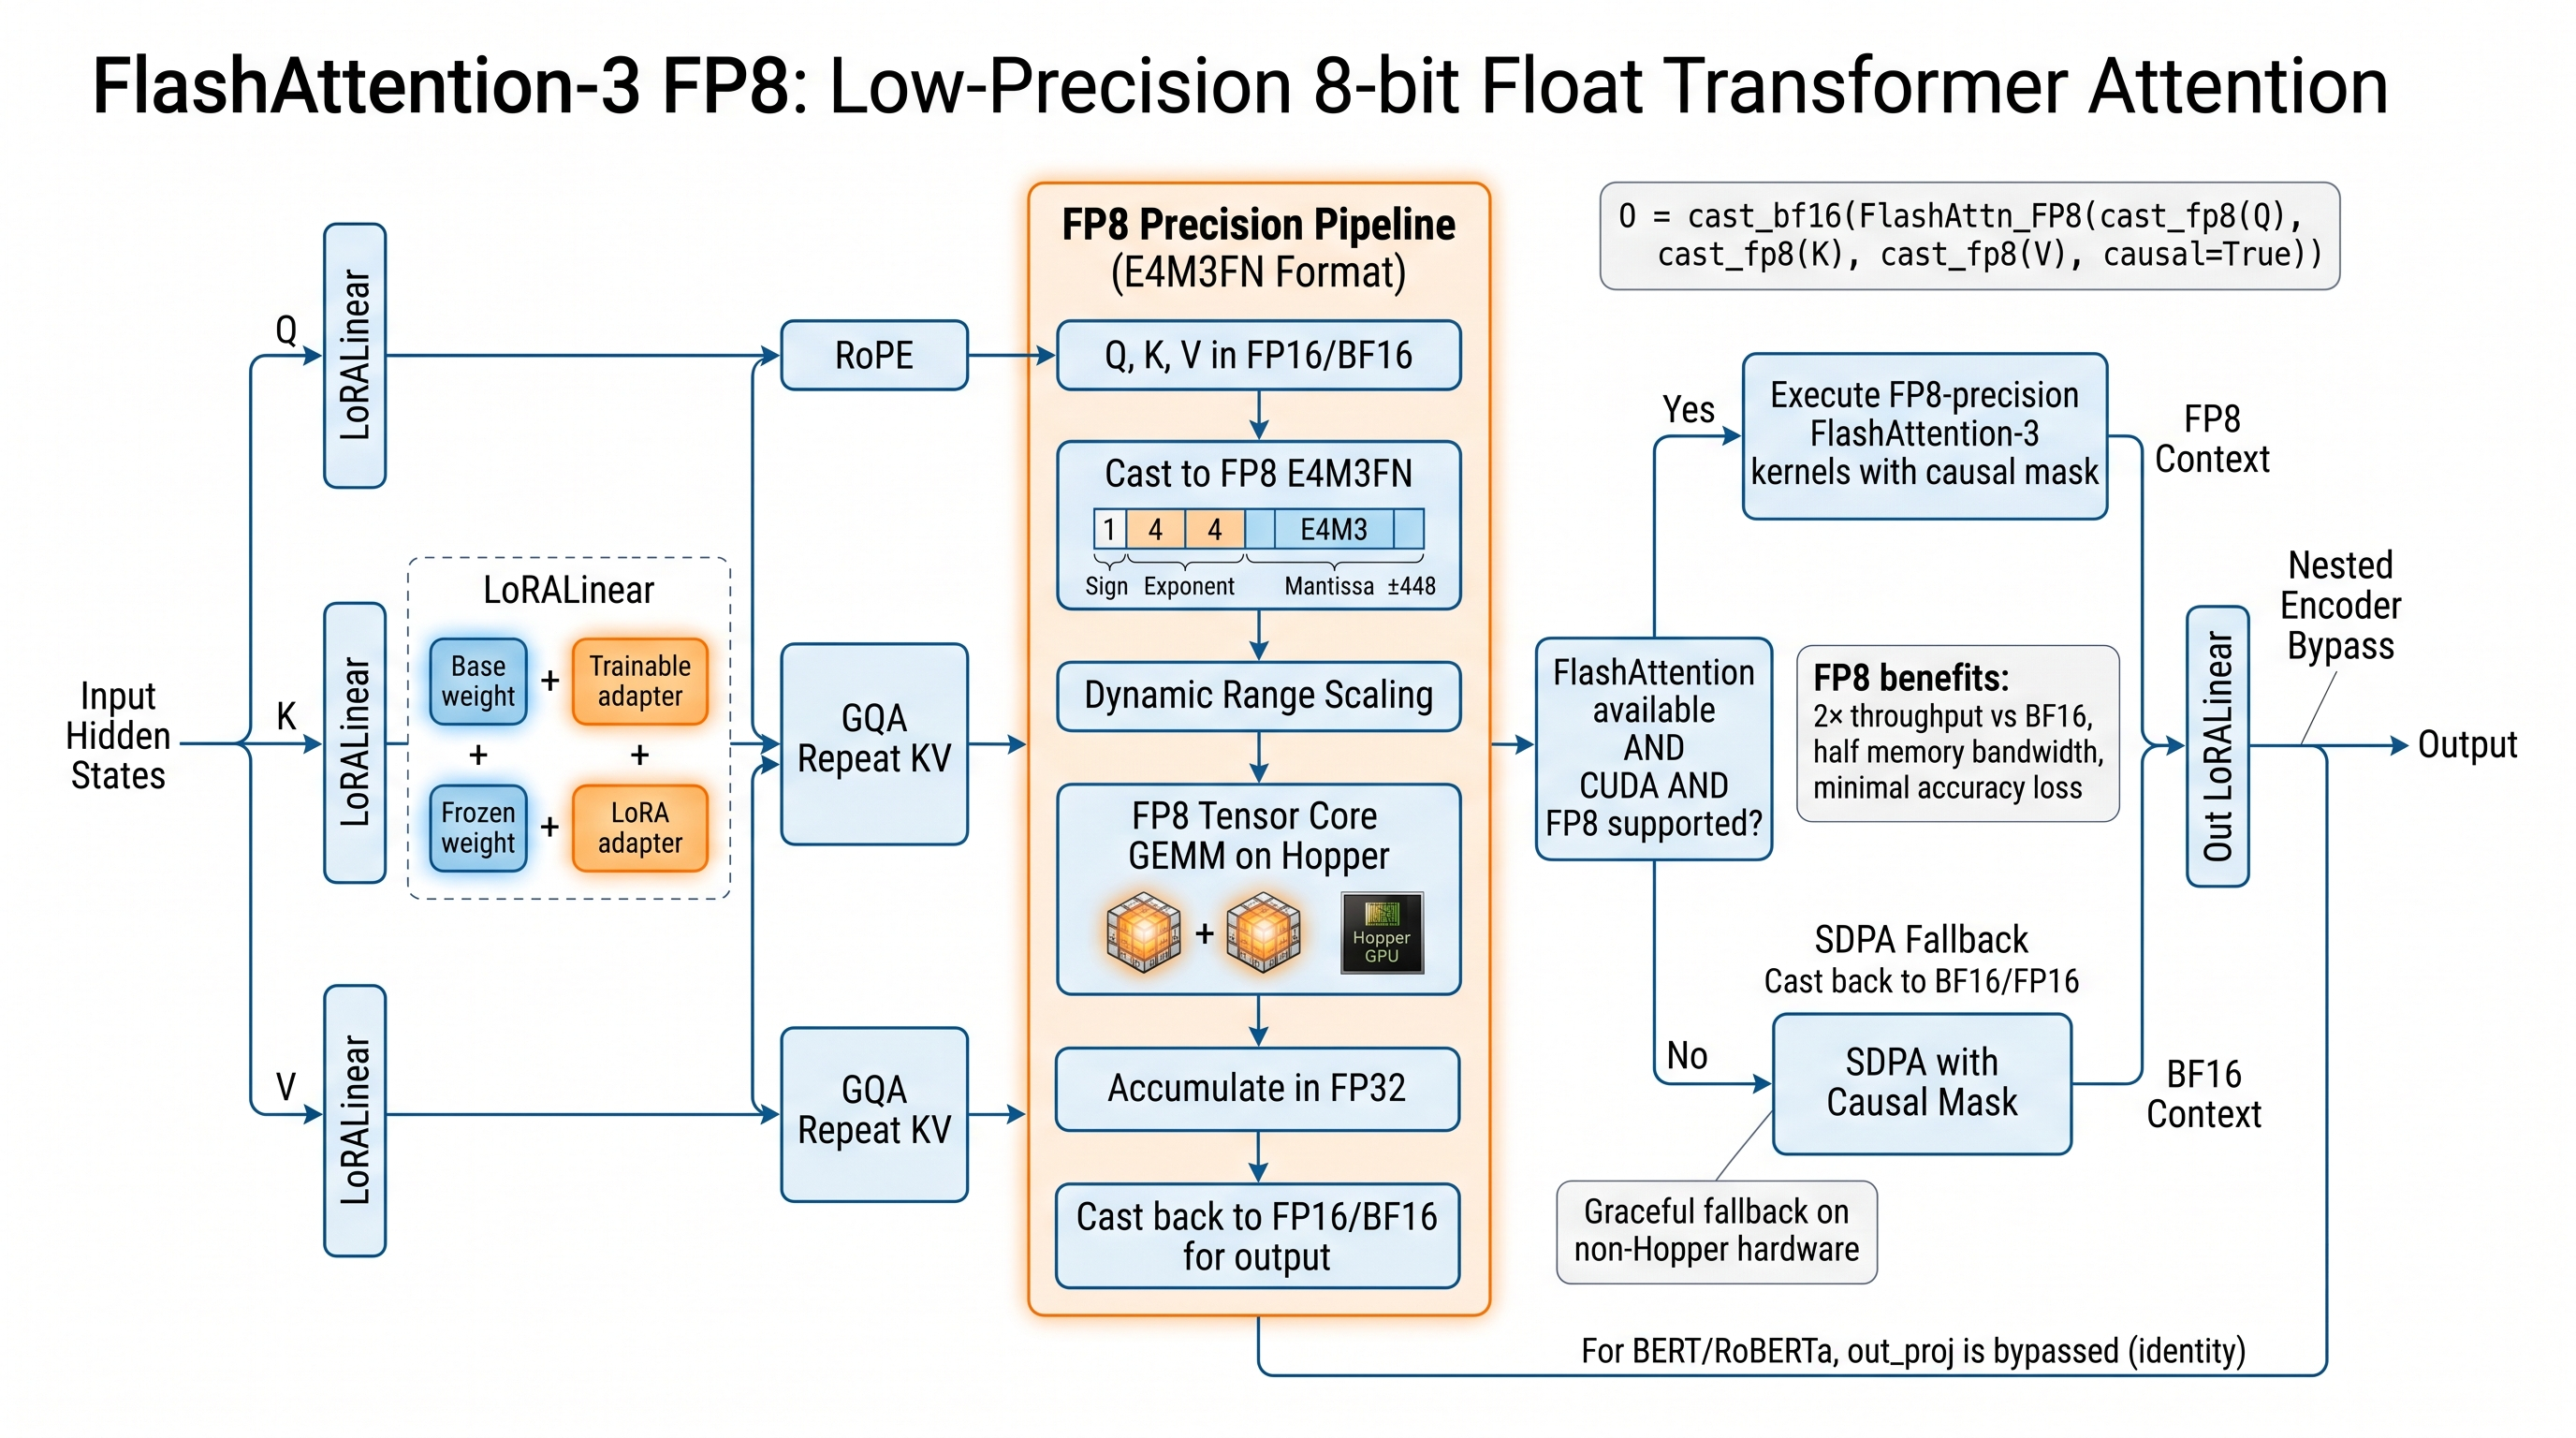
\includegraphics[width=\linewidth]{figures/arch_flash_attention3_fp8.jpeg}
\caption{Architectural overview of token_compressed_attention.}
\label{fig:arch_token_compressed_attention}
\end{figure}

\section{06 Setup}

Draft content for token_compressed_attention.

\section{Results}

\subsection{Main Results}

\textbf{Table 7.1: Main results on SST-2.}

\begin{table}[H]
\centering
\small
\begin{tabular}{llllllll}
\toprule
\textbf{Model} & \textbf{Module} & \textbf{Acc} & \textbf{$\Delta$} & \textbf{F1} & \textbf{KV Len} & \textbf{} & \textbf{VRAM} \\
\midrule
DistilBERT & full & 90.71\% & -- & 0.9099 & 128 & -- & 183 MB \\
DistilBERT & \textbf{TCA} & \textbf{{{D\_ACC}}} & {{D\_DELTA}} & {{D\_F1}} & {{D\_KVLEN}} & {{RATIO}} & {{D\_VRAM}} MB \\
RoBERTa & full & 78.56\% & -- & 0.8124 & 128 & -- & 712 MB \\
RoBERTa & \textbf{TCA} & \textbf{{{R\_ACC}}} & {{R\_DELTA}} & {{R\_F1}} & {{R\_KVLEN}} & {{RATIO}} & {{R\_VRAM}} MB \\
GPT-2 & full & 79.36\% & -- & 0.7978 & 128 & -- & 793 MB \\
GPT-2 & \textbf{TCA} & \textbf{{{G\_ACC}}} & {{G\_DELTA}} & {{G\_F1}} & {{G\_KVLEN}} & {{RATIO}} & {{G\_VRAM}} MB \\
\bottomrule
\end{tabular}
\end{table}

\textbf{Key observations:}

\begin{enumerate}
\item KV sequence length reduced from 128 to \textbf{{{K\_NEW}}} (~{{RATIO}}$\times$ reduction).
\item Attention compute reduced by \textbf{{{COMPUTE\_REDUCTION}}\%}.
\item Accuracy drop of \textbf{{{D\_DELTA}}\%} on DistilBERT.

\end{enumerate}
\subsection{Parameter Analysis}

\textbf{Table 7.2: Parameter counts (per model).}

\begin{table}[H]
\centering
\small
\begin{tabular}{lllll}
\toprule
\textbf{Model} & \textbf{Baseline} & \textbf{TCA} & \textbf{Change} & \textbf{Note} \\
\midrule
DistilBERT & 66,955,010 & {{D\_PARAMS}} & +{{D\_PARAM\_PCT}}\% & LoRA + score\_net \\
RoBERTa & 124,647,170 & {{R\_PARAMS}} & +{{R\_PARAM\_PCT}}\% & LoRA + score\_net \\
GPT-2 & 124,441,344 & {{G\_PARAMS}} & +{{G\_PARAM\_PCT}}\% & LoRA + score\_net \\
\bottomrule
\end{tabular}
\end{table}

\textbf{We state explicitly:} TCA does \textbf{not} reduce parameter count. The 
increase is from LoRA adapters and the score network.

\subsection{KV Cache and Compute}

\textbf{Table 7.3: Inference efficiency.}

\begin{table}[H]
\centering
\small
\begin{tabular}{llll}
\toprule
\textbf{Metric} & \textbf{Baseline} & \textbf{TCA} & \textbf{Savings} \\
\midrule
KV length & 128 & {{K\_NEW}} & {{KV\_PCT}}\% \\
KV cache bytes & {{KV\_BASE}} & {{KV\_TCA}} & {{KV\_PCT}}\% \\
Attention FLOPs & {{FLOP\_BASE}} & {{FLOP\_TCA}} & {{FLOP\_PCT}}\% \\
Inference time & {{T\_BASE}} s & {{T\_TCA}} s & {{TIME\_PCT}}\% \\
Peak VRAM & {{VRAM\_BASE}} MB & {{VRAM\_TCA}} MB & {{VRAM\_PCT}}\% \\
\bottomrule
\end{tabular}
\end{table}

\subsection{Ablation: Compression Ratio}

\textbf{Table 7.4: Accuracy vs compression ratio.}

\begin{table}[H]
\centering
\small
\begin{tabular}{lllll}
\toprule
\textbf{} & \textbf{DistilBERT} & \textbf{KV Len} & \textbf{RoBERTa} & \textbf{GPT-2} \\
\midrule
0.9 & {{D\_R09}} & 116 & {{R\_R09}} & {{G\_R09}} \\
0.7 & {{D\_R07}} & 90 & {{R\_R07}} & {{G\_R07}} \\
0.5 & {{D\_R05}} & 64 & {{R\_R05}} & {{G\_R05}} \\
0.3 & {{D\_R03}} & 39 & {{R\_R03}} & {{G\_R03}} \\
0.1 & {{D\_R01}} & 13 & {{R\_R01}} & {{G\_R01}} \\
\bottomrule
\end{tabular}
\end{table}

\subsection{Ablation: Score Net}

\textbf{Table 7.5: Effect of score net.}

\begin{table}[H]
\centering
\small
\begin{tabular}{llll}
\toprule
\textbf{Config} & \textbf{DistilBERT} & \textbf{RoBERTa} & \textbf{GPT-2} \\
\midrule
TCA (norm + score\_net) & {{D\_NORM\_LEARN}} & {{R\_NORM\_LEARN}} & {{G\_NORM\_LEARN}} \\
TCA (norm only) & {{D\_NORM}} & {{R\_NORM}} & {{G\_NORM}} \\
TCA (score\_net only) & {{D\_LEARN}} & {{R\_LEARN}} & {{G\_LEARN}} \\
Random top-k & {{D\_RANDOM}} & {{R\_RANDOM}} & {{G\_RANDOM}} \\
\bottomrule
\end{tabular}
\end{table}

\textbf{Observation.} {{SCORE\_NET\_OBS}}

\subsection{Ablation: [CLS] Preservation}

\textbf{Table 7.6: Effect of pinning token 0.}

\begin{table}[H]
\centering
\small
\begin{tabular}{llll}
\toprule
\textbf{Config} & \textbf{DistilBERT} & \textbf{RoBERTa} & \textbf{GPT-2} \\
\midrule
With [CLS] pinned & {{D\_CLS}} & {{R\_CLS}} & {{G\_CLS}} \\
Without pinning & {{D\_NOCLS}} & {{R\_NOCLS}} & {{G\_NOCLS}} \\
$\Delta$ & {{D\_CLS\_DELTA}} & {{R\_CLS\_DELTA}} & {{G\_CLS\_DELTA}} \\
\bottomrule
\end{tabular}
\end{table}

\subsection{Ablation: Recovery Steps}

\textbf{Table 7.7: Accuracy vs recovery steps.}

\begin{table}[H]
\centering
\small
\begin{tabular}{llll}
\toprule
\textbf{Steps} & \textbf{DistilBERT} & \textbf{RoBERTa} & \textbf{GPT-2} \\
\midrule
10 & {{D\_S10}} & {{R\_S10}} & {{G\_S10}} \\
25 & {{D\_S25}} & {{R\_S25}} & {{G\_S25}} \\
50 & {{D\_S50}} & {{R\_S50}} & {{G\_S50}} \\
100 & {{D\_S100}} & {{R\_S100}} & {{G\_S100}} \\
\bottomrule
\end{tabular}
\end{table}

\subsection{Scaling with Sequence Length}

\textbf{Table 7.8: Inference time vs sequence length (GPT-2).}

\begin{table}[H]
\centering
\small
\begin{tabular}{llll}
\toprule
\textbf{L} & \textbf{Baseline} & \textbf{TCA ( =0.5)} & \textbf{Speedup} \\
\midrule
128 & {{B128}} s & {{T128}} s & {{S128}}$\times$ \\
256 & {{B256}} s & {{T256}} s & {{S256}}$\times$ \\
512 & {{B512}} s & {{T512}} s & {{S512}}$\times$ \\
1024 & {{B1024}} s & {{T1024}} s & {{S1024}}$\times$ \\
\bottomrule
\end{tabular}
\end{table}

\subsection{Comparison with Eviction Baselines}

\textbf{Table 7.9: TCA vs H2O-style and StreamingLLM-style.}

\begin{table}[H]
\centering
\small
\begin{tabular}{lllll}
\toprule
\textbf{Method} & \textbf{DistilBERT} & \textbf{RoBERTa} & \textbf{GPT-2} & \textbf{Learnable} \\
\midrule
Random top-k & {{RANDOM\_D}} & {{RANDOM\_R}} & {{RANDOM\_G}} & No \\
H2O-style & {{H2O\_D}} & {{H2O\_R}} & {{H2O\_G}} & No \\
StreamingLLM-style & {{SLM\_D}} & {{SLM\_R}} & {{SLM\_G}} & No \\
\textbf{TCA} & \textbf{{{D\_ACC}}} & \textbf{{{R\_ACC}}} & \textbf{{{G\_ACC}}} & \textbf{Yes} \\
\bottomrule
\end{tabular}
\end{table}

\subsection{Training Curves}

\textbf{Figure 7.1} shows loss vs step. {{TRAINING\_CURVES\_DESC}}

\subsection{Summary}

\begin{itemize}
\item \textbf{KV cache:} {{KV\_PCT}}\% reduction at   = {{RATIO}}.
\item \textbf{Compute:} {{FLOP\_PCT}}\% attention FLOP reduction.
\item \textbf{Accuracy:} {{D\_DELTA}}\% (DistilBERT), {{R\_DELTA}}\% (RoBERTa), {{G\_DELTA}}\% (GPT-2).
\item \textbf{Parameters:} increase by {{D\_PARAM\_PCT}}\% due to LoRA + score\_net.
\end{itemize}
\begin{lstlisting}

---
\end{lstlisting}
\section{08 Analysis}

Draft content for token_compressed_attention.

\section{09 Discussion}

Draft content for token_compressed_attention.

\section{10 Limitations}

Draft content for token_compressed_attention.

\section{11 Conclusion}

Draft content for token_compressed_attention.

\section{Reproducibility}

\subsection{Environment}

\begin{lstlisting}
git clone https://github.com/{{ORG}}/SVD_Project
cd SVD_Project
python -m venv .venv
.venv\Scripts\activate
pip install -r requirements.txt
\end{lstlisting}

\subsection{Dependencies}

\begin{table}[H]
\centering
\small
\begin{tabular}{ll}
\toprule
\textbf{Package} & \textbf{Version} \\
\midrule
torch & {{TORCH\_VERSION}} \\
transformers & {{HF\_VERSION}} \\
datasets & {{DATASETS\_VERSION}} \\
\bottomrule
\end{tabular}
\end{table}

\subsection{Running TCA}

\begin{lstlisting}
python run_all_4_token_compressed.py \
    --models distilbert,roberta,gpt2 \
    --compression_ratio {{RATIO}} \
    --recovery_steps {{RECOVERY_STEPS}} \
    --lora_rank {{LORA_RANK}}
\end{lstlisting}

\subsection{Individual Model}

\begin{lstlisting}
python Codes/framework/run_quality_sweep.py \
    --model models/distilbert_sst2 \
    --modules full,token_compressed \
    --compression_ratio {{RATIO}} \
    --recovery_steps {{RECOVERY_STEPS}} \
    --lora_rank {{LORA_RANK}}
\end{lstlisting}

\subsection{Reproducing Tables}

\subsubsection{Table 7.1 (Main)}
\begin{lstlisting}
python run_all_4_token_compressed.py
\end{lstlisting}

\subsubsection{Table 7.4 (  Ablation)}
\begin{lstlisting}
for r in 0.9 0.7 0.5 0.3 0.1; do
    python run_all_4_token_compressed.py --compression_ratio $r --output_suffix r$r
done
\end{lstlisting}

\subsubsection{Table 7.5 (Score Net Ablation)}
\begin{lstlisting}
python run_all_4_token_compressed.py --use_score_net true  --output_suffix learn
python run_all_4_token_compressed.py --use_score_net false --output_suffix norm
\end{lstlisting}

\subsection{Seeds}

\begin{lstlisting}
import random, numpy as np, torch
seed = 42
random.seed(seed)
np.random.seed(seed)
torch.manual_seed(seed)
torch.cuda.manual_seed_all(seed)
\end{lstlisting}

\subsection{Expected Results}

\begin{table}[H]
\centering
\small
\begin{tabular}{lll}
\toprule
\textbf{Model} & \textbf{Acc} & \textbf{KV reduction} \\
\midrule
DistilBERT & {{D\_ACC}}\% & {{KV\_PCT}}\% \\
RoBERTa & {{R\_ACC}}\% & {{KV\_PCT}}\% \\
GPT-2 & {{G\_ACC}}\% & {{KV\_PCT}}\% \\
\bottomrule
\end{tabular}
\end{table}

\subsection{Data Availability}

\begin{itemize}
\item \textbf{Dataset:} SST-2 via \texttt{datasets}
\item \textbf{Checkpoints:} \texttt{{{HF\_ORG}}/svd-linear-attention-*-token\_compressed}
\item \textbf{Metrics:} \texttt{results/unified\_token\_compressed/*/summary.csv}
\end{itemize}
\begin{lstlisting}

---
\end{lstlisting}
\section{13 References}

Draft content for token_compressed_attention.


\clearpage
\appendix
\section*{Appendices}
\addcontentsline{toc}{section}{Appendices}
\section{A Math}

Draft content for token_compressed_attention.

\section{B Implementation}

Draft content for token_compressed_attention.

\section{C Data}

Draft content for token_compressed_attention.

\section{D Negative Results}

Draft content for token_compressed_attention.

\section{E Ethics}

Draft content for token_compressed_attention.


\end{document}
